%%%%%%%%%%%%%%%%%%%%%%%%%%%%%%%%%%%%%%%%%%%%%%%%%%%%%%%%%%%
% Vorlage f. Abschlussarbeiten														%
%	Hochschule Bochum, it:matters														%
% MIRo-Lab																								%
%	Autor:		Dr. Sven Seiler <sven.seiler@hs-bochum.de>		%
%																													%
%Fr�here Autoren:																					%
%						Martin B�lter	<martin.boelter@hs-bochum.de>		%
%						Jens Jakobi	<jens.jakobi@hs-bochum.de>				%
%																													%
%																													%
% Version: 0.91, 07-02-2013																%
%%%%%%%%%%%%%%%%%%%%%%%%%%%%%%%%%%%%%%%%%%%%%%%%%%%%%%%%%%%

%
% F�r diese Vorlage �bernehmen die Autoren keine Gew�hr.
% Bitte kl�ren Sie mit Ihren Pr�fern ab, ob und in welcher
% Form Sie diese Vorlage f�r Ihre Arbeit verwenden d�rfen.
\newcommand{\DeinName}{Anthony Mendil}
\newcommand{\TitelArbeit}{Using bevavioural data and brain activity to determine whether players were blinded during a game of memory}
\newcommand{\Labor}{Cognitive Systems Lab (CSL)}
\newcommand{\PrueferEins}{Dr. Felix Putze}
\newcommand{\PrueferZwei}{Unknown}
\newcommand{\Supervisor}{Mazen Salous}
\newcommand{\fachbereich}{Mathematics and Computer Science}
% entweder ein Datum h�ndisch eintragen, oder den Befehl \today nutzen
\newcommand{\Datum}{\today}

\makeglossary


%
% Einbinden des Headers, hier k�nnen auch weitere Einstellungen vorgenommen werden.
%%%%%%%%%%%%%%%%%%%%%%%%%%%%%%%%%%%%%%%%%%%%%%%%%%%%%%%
%																					%
%	In dieser Datei werden alle Packages eingebunden, 	%
% welche f�r das Dokument n�tig sind. Desweiteren 		%
% werden die Dokumentinformationen gesetzt.						%
%																											%
%%%%%%%%%%%%%%%%%%%%%%%%%%%%%%%%%%%%%%%%%%%%%%%%%%%%%%%
%
%	Die KOMAScript Dokumentklasse "scrbook" verwenden.
%
\documentclass[pdftex, 		%
							a4paper, 		% DIN A4 verwenden
							titlepage,	% separate Titelseite
							%draft,			%	Draft-Version, keine Bilder im pdf!
							final,			% Final-Version
							oneside,		% einseitiger Druck
							11pt,				% Schriftgr��e 12pt
							DIV=calc,
							%tocbasic,
							]{scrbook}	%	KOMAScript scrbook-Dokumentklasse
							
%%%%%%%%%%%%%%%%%%%%%%%%%%%%%%%%%%%%%%%%%%%%%%%%%%%%%%%%
%	Einbinden der Pakete 
%%%%%%%%%%%%%%%%%%%%%%%%%%%%%%%%%%%%%%%%%%%%%%%%%%%%%%%%

\usepackage[ngerman]{babel}

% PDF Dateien einbinden
\usepackage{pdfpages}

%Settings for PDF Pages to accept additonal versioned PDF files
\pdfminorversion=6
\pdfcompresslevel=9
\pdfobjcompresslevel=9

%Infos dazu unter: http://www.bakoma-tex.com/doc/latex/koma-script/scrhack.pdf
%Einige Pakete haben Probleme mit dem Komaskript.
\usepackage{scrhack} 


% Definieren von eigenen benannten Farben.
% F�r sp�tere Verwendung in dem Dokument, definieren wir einzelne
% benannte Farben.
%
\usepackage{xcolor}
\definecolor{gray1}{gray}{0.92}
\definecolor{darkgreen}{rgb}{0,0.5,0}

\definecolor{urlLinkColor}{rgb}{0,0,0.5}
\definecolor{LinkColor}{rgb}{0,0,0}
\definecolor{ListingBackground}{rgb}{0.85,0.85,0.85}




\rmfamily
\usepackage{natbib}
\usepackage{palatino} 				% Schriftfamilie Palatino
\usepackage[latin1]{inputenc} % Umlaute  
%\usepackage[dvips]{color}    	% f�r graue Boxen
%\usepackage[dvips]{graphicx} 	% Grafikpaket
\usepackage{makeidx}   				% Paket zur Erzeugung eines Index
\usepackage[normalem]{ulem}   % bietet Unterstreichungsvarianten
\usepackage{picins} 					% Bilder im Absatz platzieren
\usepackage[T1]{fontenc}			% Erweiterten Zeichensatz aktivieren
\usepackage{multido}					% erm�glicht Schleifenartiges wiederholen von Befehlen
\usepackage{mdwlist}					% erm�glicht das Setzen des Z�hlers bei Aufz�hlungspunkten
\usepackage{paralist}					% Paket f�r Aufz�hlungen, erweitert Enumerate-Paket
\usepackage{longtable}				% mehrseitige Tabellen
\usepackage{tocbasic}
\parindent0pt           			% verzichte auf Einr�cken der ersten Zeile
\parskip1ex             			% Abstand zwischen den Abs�tzen

\usepackage{setspace}					% Paket zum Einstellen des Zeilenabstands
\onehalfspacing								% anderthalbfacher Zeilenabstand
%\doublespacing								% doppelter Zeilenabstand
%\singlespacing								% einfacher Zeilenabstand

%\usepackage[german]{babel}
\usepackage[german=quotes]{csquotes} %Deutsche Anf�hrungszeichen

\usepackage{color}
\definecolor{LinkColor}{rgb}{0.1,0.1,0.1}
%\definecolor{ListingBackground}{rgb}{0.85,0.85,0.85}
\definecolor{ListingBackground}{rgb}{0.98,0.98,0.98}
\definecolor{gray}{rgb}{0.4,0.4,0.4}
\definecolor{darkblue}{rgb}{0.0,0.0,0.6}
\definecolor{cyan}{rgb}{0.0,0.6,0.6}


\usepackage{geometry}
\geometry{
	a4paper,
	total={170mm,257mm},
	left=20mm,
	top=20mm,
}

%
% Farbeinstellungen f�r die Links im PDF Dokument.
%
\makeindex

%-----------Paket f�r absolute Positionierung von Grafiken------------------
\usepackage[absolute]{textpos}
\setlength{\TPHorizModule}{1mm}
\setlength{\TPVertModule}{\TPHorizModule}

%-----------Aufz�hlungen und Einstellungen f�r Sourcecode-------------------
%\usepackage[savemem]{listings} %Bei wenig Arbeitsspeicher dies Option [savemem] aktivieren.
\usepackage{listings}
\lstloadlanguages{TeX,XML, Java} % TeX sprache laden, notwendig wegen option 'savemem'
\lstset{%
	language=[LaTeX]TeX,     % Sprache des Quellcodes ist TeX
	numbers=left,            % Zelennummern links
	stepnumber=1,            % Jede Zeile nummerieren.
	numbersep=5pt,           % 5pt Abstand zum Quellcode
	numberstyle=\tiny,       % Zeichengr�sse 'tiny' f�r die Nummern.
	breaklines=true,         % Zeilen umbrechen wenn notwendig.
	breakautoindent=true,    % Nach dem Zeilenumbruch Zeile einr�cken.
	postbreak=\space,        % Bei Leerzeichen umbrechen.
	tabsize=2,               % Tabulatorgr�sse 2
	basicstyle=\ttfamily\footnotesize, % Nichtproportionale Schrift, klein f�r den Quellcode
	showspaces=false,        % Leerzeichen nicht anzeigen.
	showstringspaces=false,  % Leerzeichen auch in Strings ('') nicht anzeigen.
	extendedchars=true,      % Alle Zeichen vom Latin1 Zeichensatz anzeigen.
	backgroundcolor=\color{ListingBackground}} % Hintergrundfarbe des Quellcodes setzen.


\lstset{
  basicstyle=\small\ttfamily,
  columns=fullflexible,
  showstringspaces=false,
  %commentstyle=\color{gray}\upshape
}
%neue Lang definieren, als Bsp.
\lstdefinelanguage{XML-changed}
{
  basicstyle=\footnotesize\ttfamily\bfseries,
  morestring=[b]",
  morestring=[s]{>}{<},
  morecomment=[s]{<?}{?>},
  stringstyle=\color{black},
  identifierstyle=\color{darkblue},
  keywordstyle=\color{cyan},
  morekeywords={xmlns,version,type}% list your attributes here
}

%-----------Caption Package-------------------
\usepackage{caption}
\DeclareCaptionFont{white}{\color{white}}
\DeclareCaptionFormat{listing}{\colorbox[cmyk]{0.43, 0.35, 0.35,0.01}{\parbox{\textwidth}{\hspace{15pt}#1#2#3}}}

\DeclareCaptionFormat{graphics}{\colorbox[cmyk]{0.43, 0.35, 0.35,0.01}{\parbox{\textwidth}{\hspace{15pt}#1#2#3}}}


\captionsetup[lstlisting]{format=listing,labelfont=white,textfont=white, singlelinecheck=false, margin=0pt, font={footnotesize}}

%-----------Header+Footer---------------------------------------------------
\usepackage{fancyhdr}					%
\pagestyle{fancy}							%

\fancyhead{}
\fancyfoot{} 
\renewcommand{\headrulewidth}{0.4pt} % Kopzeilenlinie
\renewcommand{\footrulewidth}{0.0pt} % Fusszeilenlinie 0.0pt blendet sie aus

\renewcommand{\chaptermark}[1]{\markboth{\thechapter\quad#1}{}}
\renewcommand{\sectionmark}[1]{\markright{\thesection\quad#1}}

\fancyhead[LO]{\small\sffamily\rightmark}
\fancyhead[RO]{\small\sffamily\thepage}

%-----------Um die Eidesstattliche Erkl�rung als PDF einzubinden-----------------------------------
%\usepackage{pdfpages}

%------------Glossar--------------------------------------------------------------
\usepackage{expdlist}
\usepackage{glossar}

\renewcommand{\glshead}{\chapter*{Glossar}}
\renewcommand{\glentry}[2]{\glossary{#1@[#1] #2|glspage}}
\renewcommand{\glsgroup}[1]{{\listpart{\makebox[0pt][l]{\rule[-2pt]{\textwidth}{0.5pt}}{\textbf{\large #1}}}}}

\makeglossary

%Glossar mit Bordmitteln ------------------------------------------------------------------
%Darstellung des Glossars einstellen
%\usepackage[style=super, header=none, border=none, number=none, cols=2, toc=true]{glossary}
%\renewcommand{\glossaryname}{Glossar}
%\printglossary

% --- diverse Schriften -------------------------------------------------------------------
%\newcommand{\url}[1]{{\sf\small #1}}     % Hyperlinks


% -------F�r ToDo-Notes--------------------------------------------------------------------
\usepackage[color=red, shadow]{todonotes} % ", disable" deaktiviert ToDo-Notes
%Vereinfachtes "Inline-Todo"
\newcommand{\td}[1]{{\todo[inline]{#1}}}
\newcommand{\tdu}[1]{{\todo[inline, color=green!40]{#1}}}

%--------F�r Links-------------------------------------------------------------------------




%--------HyperRef konfigurieren-------------------------------------------------------------------------

\usepackage[
	pdftitle={\TitelArbeit},
	pdfauthor={\DeinName},
	pdfsubject={\TitelArbeit},
	pdfcreator={MiKTeX, LaTeX with hyperref and KOMA-Script auf Basis der Vorlage von seiler.it},
	pdfkeywords={Abschlussarbeit, Bochum, Hoschule},%weitere Keywords hier einf�gen
	pdfpagemode=UseOutlines,%                                  
	pdfdisplaydoctitle=true,%                                  
	pdflang=de%                                              
]{hyperref}

\hypersetup{%
	colorlinks=true,%        Aktivieren von farbigen Links im Dokument (keine Rahmen)
	linkcolor=LinkColor,%    Farbe festlegen.
	citecolor=LinkColor,%    Farbe festlegen.
	filecolor=LinkColor,%    Farbe festlegen.
	menucolor=LinkColor,%    Farbe festlegen.
	urlcolor=LinkColor,%     Farbe von URL's im Dokument.
	bookmarksnumbered=true%  �berschriftsnummerierung im PDF Inhalt anzeigen.
}



% Beginn des Dokuments
\begin{document}


%Zitiert alle Referenzen, ohne Sie hier zu listen. Dadurch erscheinen alle Quellen im %Literaturverzeichnis, auch wenn sie im Text nicht genutzt werden.
%Bitte nur f�r Testzwecke verwenden.
\nocite{*}


% Einbinden des Deckblatts

\frontmatter
% erste Seite (Titelseite) der Diplomarbeit mit Titel, Name usw...

\newsavebox{\Prof}
\savebox{\Prof}{Erster Pr�fer }

\newsavebox{\Betr}
\savebox{\Betr}{Zweiter Pr�fer }

\newsavebox{\Examiner}
\savebox{\Examiner}{}



\begin{titlepage}
%\begin{textblock}{50}(150,30)
  %
\includegraphics[height=3cm]{source/images/BO-Logo_m_Wortmarke_P10cmWebHQ}
	%
\includegraphics[height=1cm]{source/images/BO-Logo_m_Wortmarke_L10cmWebHQ}	
%	
\includegraphics[height=4cm]{source/images/BO-Logo_m_Wortmarke_P10cmWebHQ}
%\end{textblock}
\begin{center}
%
\includegraphics[height=2cm]{source/images/logo_mirolab.png}

{\large University of Bremen}\\[1mm]
{\small Faculty: \fachbereich}\\
{\small Computer Science Bachelor}
\vspace{1.5cm}

{\huge \TitelArbeit}

\vspace{1,5cm}

{\large Bachelor Thesis}

\vspace{1cm}

by\\[2mm]

\textbf{\large{\DeinName}}\\

\vspace{1cm}
\Labor\\[1cm]

Examiner: \\[2mm]

\usebox{\Examiner \PrueferEins} \\
\usebox{\Examiner \PrueferZwei} \\

\vspace{1cm}

Supervisor: \\[2mm]

\usebox{\Examiner \Supervisor} \\

\vspace{1cm}
Bremen, date 
\end{center}
\begin{textblock}{50}(30,250)
  %
\includegraphics[height=3cm]{source/images/BO-Logo_m_Wortmarke_P10cmWebHQ}
	
\includegraphics[height=1cm]{source/images/uni_logo}	
	
\end{textblock}

%% Hier kann nat�rlich auch jedes andere Logo eingebunden werden! %%
\begin{textblock}{40}(142,248)
  
\includegraphics[height=1.5cm]{source/images/csl_logo}
\end{textblock}
\end{titlepage}



\chapter{Eidesstattliche Erkl�rung}
Hiermit erkl�re ich, \DeinName, die vorliegende Diplomarbeit selbstst�ndig und nur unter Verwendung der von mir angegebenen Literatur verfasst zu haben. 

Die aus fremden Quellen direkt oder indirekt �bernommenen Gedanken sind als solche kenntlich gemacht.

Diese Arbeit hat in gleicher oder �hnlicher Form keiner anderen Pr�fungsbeh�rde vorgelegen.\\
\\[6ex]

Bochum, den \today


\rule[-0.2cm]{5cm}{0.5pt}

\textsc{\DeinName} 

\todo[inline]{Eidesstattliche Erkl�rung vom Pr�fungsamt benutzen! Und diese Seite wieder ganz ausschlie�en!}
%
% EOF
%

%\includepdf[noautoscale=true]{source/content/Deckblatt_der_Diplomarbeit0901.pdf}

% Der Abstract, bitte in englischer Sprache verfassen!
\chapter{Abstract}
\label{Abstract}
Der Abstract sollte auf Englisch verfasst werden. Er ist eine komprimierte Wiedergabe der wesentlichen Erkentnisse die w�hrend der Abschlussarbeitsphase gewonnen wurden. Der Abstract soll dem Leser eine Entscheidungsgrundlage liefern, ob der Text f�r ihn/sie interessant und lesenswert ist.
\\
\todo[inline]{Der Abstract sollte zum Ende der Arbeit geschrieben werden...}
Lorem ipsum dolor sit amet, consetetur sadipscing elitr, sed diam nonumy eirmod tempor invidunt ut labore et dolore magna aliquyam erat, sed diam voluptua. At vero eos et accusam et justo duo dolores et ea rebum. Stet clita kasd gubergren, no sea takimata sanctus est Lorem ipsum dolor sit amet. Lorem ipsum dolor sit amet, consetetur sadipscing elitr, sed diam nonumy eirmod tempor invidunt ut labore et dolore magna aliquyam erat, sed diam voluptua. At vero eos et accusam et justo duo dolores et ea rebum. Stet clita kasd gubergren, no sea takimata sanctus est Lorem ipsum dolor sit amet. Lorem ipsum dolor sit amet, consetetur sadipscing elitr, sed diam nonumy eirmod tempor invidunt ut labore et dolore magna aliquyam erat, sed diam voluptua. At vero eos et accusam et justo duo dolores et ea rebum. Stet clita kasd gubergren, no sea takimata sanctus est Lorem ipsum dolor sit amet. 
Lorem ipsum dolor sit amet, consetetur sadipscing elitr, sed diam nonumy eirmod tempor invidunt ut labore et dolore magna aliquyam erat, sed diam voluptua. At vero eos et accusam et justo duo dolores et ea rebum. Stet clita kasd gubergren, no sea takimata sanctus est Lorem ipsum dolor sit amet. Lorem ipsum dolor sit amet,  


% Einbinden des Inhaltsverzeichnisses
%\todo[inline]{Inhaltsverzeichnis-Schachtelungswerte auf Standard zur�cksetzen!}
%\setcounter{secnumdepth}{4} % Schachtelungstiefe der Nummerierung von �berschriften
%\setcounter{tocdepth}{4} % Schachtelungstiefe des Inhaltsverzeichnisses
\tableofcontents 

%Einbinden des Hauptteils
\mainmatter

\begin{table}
	\centering
	\caption{2D CNN. 20 turns. config2}%\label{tab1}
	\begin{tabular}{|l|l|l|}
		\hline
		Simulated Games & Best Accuracy (Epoch) & Best Loss (Epoch)\\
		\hline
		0 & 0.7888 (14) & 0.4822 (51) \\
		1 &  &  \\
		2 &  &  \\
		3 &  &  \\
		4 &  &  \\
		5 & 0.8450 (17) & 0.4768 (20) \\
		6 &  &  \\
		7 &  &  \\
		8 &  &  \\
		9 &  &  \\
		10 & 0.8475 (20) & 0.4796 (10) \\
		20 & 0.8437 (6) & 0.4763 (6) \\
		\hline
	\end{tabular}
\end{table}

\begin{table}
	\centering
	\caption{2D CNN. 20 turns. config1}%\label{tab1}
	\begin{tabular}{|l|l|l|}
		\hline
		Simulated Games & Best Accuracy (Epoch) & Best Loss (Epoch)\\
		\hline
		0 & 0.7963 (18) & 0.4931 (98) \\
		1 &  &  \\
		2 &  &  \\
		3 &  &  \\
		4 &  &  \\
		5 & 0.8437 (53) & 0.4821 (31) \\
		6 &  &  \\
		7 &  &  \\
		8 &  &  \\
		9 &  &  \\
		10 &  &  \\
		20 &  &  \\
		\hline
	\end{tabular}
\end{table}



\chapter{Einleitung}
\section{Motivation}
Hier sollten die folgenden Fragestellungen bearbeitet werden:

\begin{itemize}
	\item Warum soll das Thema bearbeitet werden, was war der ausschlaggebende Grund dazu?
	\item Gibt es vll. geleistete Vorarbeit aus Labort�tigkeit, oder wurde das Thema von einem Betreuuer vorgeschlagen?
	\item In welchem Kontext steht das Thema zur akademische Ausbildung?
	\item Warum ist es sinnvoll das Thema zu bearbeiten?
\end{itemize}

\section{Aufgabenstellung}
Wie lautet die Aufgabenstellung?
\todo[inline]{Hier muss noch die Aufgabenstellung erg�nzt werden!}

Lorem ipsum dolor sit amet, consetetur sadipscing elitr, sed diam nonumy eirmod tempor invidunt ut labore et dolore magna aliquyam erat, sed diam voluptua. At vero eos et accusam et justo duo dolores et ea rebum. Stet clita kasd gubergren, no sea takimata sanctus est Lorem ipsum dolor sit amet. Lorem ipsum dolor sit amet, consetetur sadipscing elitr, sed diam nonumy eirmod tempor invidunt ut labore et dolore magna aliquyam erat, sed diam voluptua. At vero eos et accusam et justo duo dolores et ea rebum. Stet clita kasd gubergren, no sea takimata sanctus est Lorem ipsum dolor sit amet. Lorem ipsum dolor sit amet, consetetur sadipscing elitr, sed diam nonumy eirmod tempor invidunt ut labore et dolore magna aliquyam erat, sed diam voluptua. At vero eos et accusam et justo duo dolores et ea rebum. Stet clita kasd gubergren, no sea takimata sanctus est Lorem ipsum dolor sit amet. 
Lorem ipsum dolor sit amet, consetetur sadipscing elitr, sed diam nonumy eirmod tempor invidunt ut labore et dolore magna aliquyam erat, sed diam voluptua. At vero eos et accusam et justo duo dolores et ea rebum. Stet clita kasd gubergren, no sea takimata sanctus est Lorem ipsum dolor sit amet. Lorem ipsum dolor sit amet, consetetur sadipscing elitr, sed diam nonumy eirmod tempor invidunt ut labore et dolore magna aliquyam erat, sed diam voluptua. At vero eos et accusam et justo duo dolores et ea rebum. Stet clita kasd gubergren, no sea takimata sanctus est Lorem ipsum dolor sit amet. Lorem ipsum dolor sit amet, consetetur sadipscing elitr, sed diam nonumy eirmod tempor invidunt ut labore et dolore magna aliquyam erat, sed diam voluptua. At vero eos et accusam et justo duo dolores et ea rebum. Stet clita kasd gubergren, no sea takimata sanctus est Lorem ipsum dolor sit amet. 
Lorem ipsum dolor sit amet, consetetur sadipscing elitr, sed diam nonumy eirmod tempor invidunt ut labore et dolore magna aliquyam erat, sed diam voluptua. At vero eos et accusam et justo duo dolores et ea rebum. Stet clita kasd gubergren, no sea takimata sanctus est Lorem ipsum dolor sit amet. Lorem ipsum dolor sit amet, consetetur sadipscing elitr, sed diam nonumy eirmod tempor invidunt ut labore et dolore magna aliquyam erat, sed diam voluptua. At vero eos et accusam et justo duo dolores et ea rebum. Stet clita kasd gubergren, no sea takimata sanctus est Lorem ipsum dolor sit amet. Lorem ipsum dolor sit amet, consetetur sadipscing elitr, sed diam nonumy eirmod tempor invidunt ut labore et dolore magna aliquyam erat, sed diam voluptua. At vero eos et accusam et justo duo dolores et ea rebum. Stet clita kasd gubergren, no sea takimata sanctus est Lorem ipsum dolor sit amet. 



\chapter{Problemstellung und Stand der Technik}
\section{Erster Abschnitt}
	\subsection{Aufz�hlungen}
\todo[inline]{Hier Punkte die zu erledigen sind}

\begin{itemize}
	\item Dies
	\item[\dots] ist eine 
	\item Aufz�hlung
\end{itemize}

\begin{enumerate}
	\item Dies
	\item ist eine nummerierte
	\item Aufz�hlung
\end{enumerate}

Weitere Infos u.a. auf:\\
\url{http://de.wikibooks.org/wiki/LaTeX-W%C3%B6rterbuch:_Aufz%C3%A4hlung}\\

\subsection{Minipages}
\begin{minipage}[h!][9cm][t]{3cm}
	Dies ist ein Beispieltext innerhalb einer Minipage. Diese Minipage ist 4cm breit und 59cm hoch	
\end{minipage}

So sieht die generelle Anweisung aus:
\begin{verbatim}
	\begin{minipage}[�USSERE POSITION][H�HE][INNERE POSITION]{BREITE}
	Beispieltext
  \end{minipage}
\end{verbatim}
Weitere Infos u.a. auf:\\
\url{http://www.golatex.de/wiki/minipage}\\
\url{http://www.weinelt.de/latex/minipage.html}\\
\url{http://www.namsu.de/Extra/befehle/Minipage.html}\\

Lorem ipsum dolor sit amet, consetetur sadipscing elitr, sed diam nonumy eirmod tempor invidunt ut labore et dolore magna aliquyam erat, sed diam voluptua. At vero eos et accusam et justo duo dolores et ea rebum. Stet clita kasd gubergren, no sea takimata sanctus est Lorem ipsum dolor sit amet. Lorem ipsum dolor sit amet, 

\section{Grafiken}
Nachfolgend ein paar Beispiele zum Einbinden von Grafiken.
Weitere Infos u.a. auf:\\
\url{ftp://ftp.dante.de/tex-archive/info/l2picfaq/german/l2picfaq.pdf}\\
\url{http://latex.mschroeder.net/}\\
\url{http://latex.hpfsc.de/content/latex_tutorial/grafiken}\\
\url{http://de.wikibooks.org/wiki/LaTeX-Kompendium:_Schnellkurs:_Grafiken}\\

\begin{figure}
\centering
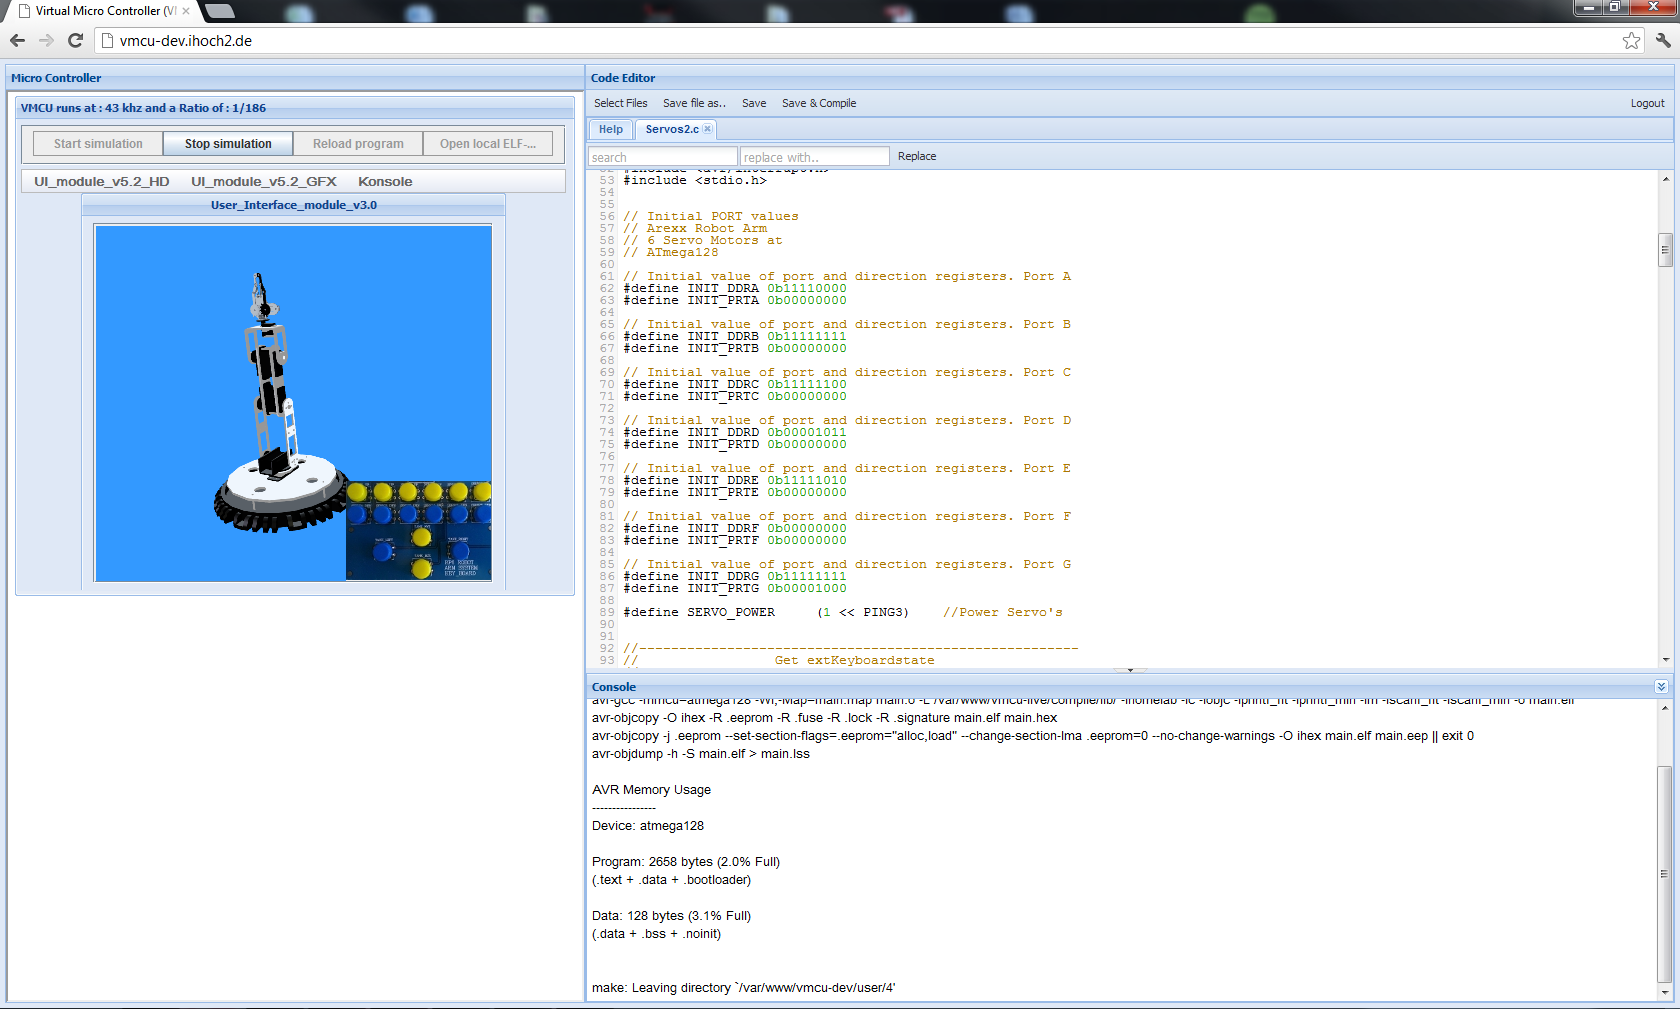
\includegraphics[width=0.2\textwidth]{source/images/vmcu-env}
\caption{Breite entspricht der 20\% d. Textweite}
\label{fig:vmcu:overview1}
\end{figure}

\begin{figure}
\centering
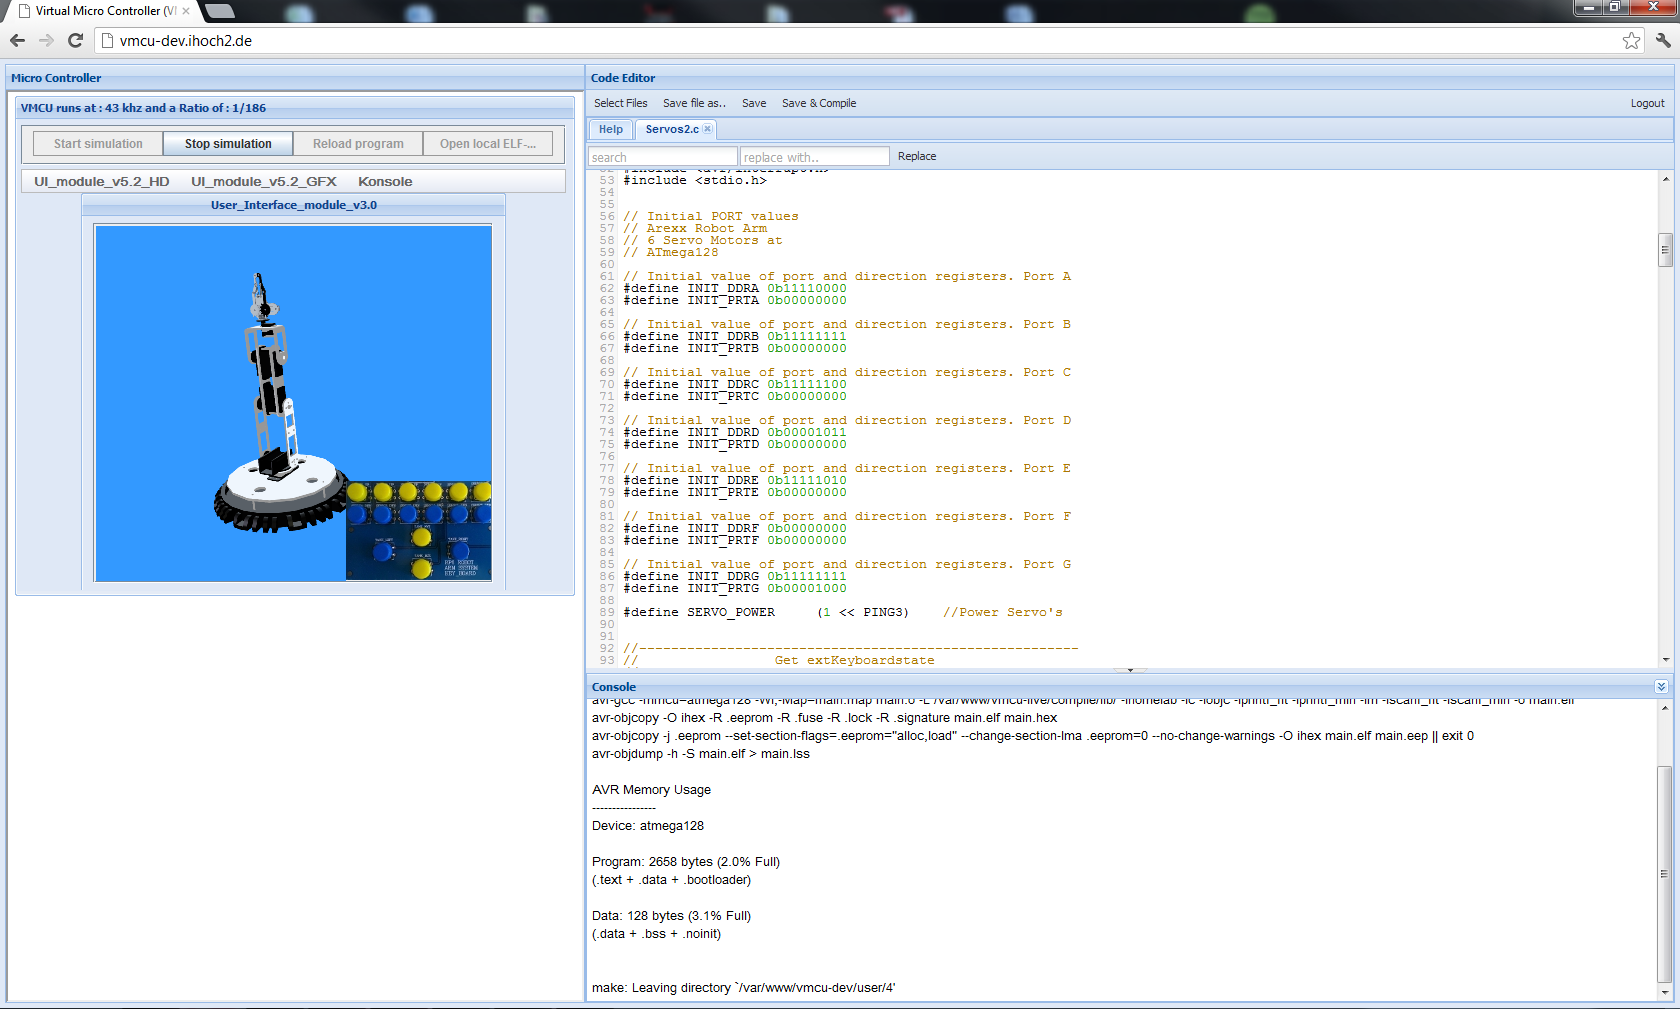
\includegraphics[width=8cm]{source/images/vmcu-env}
\caption{8cm breit}
\label{fig:vmcu:overview2}
\end{figure}


\begin{figure}
\centering
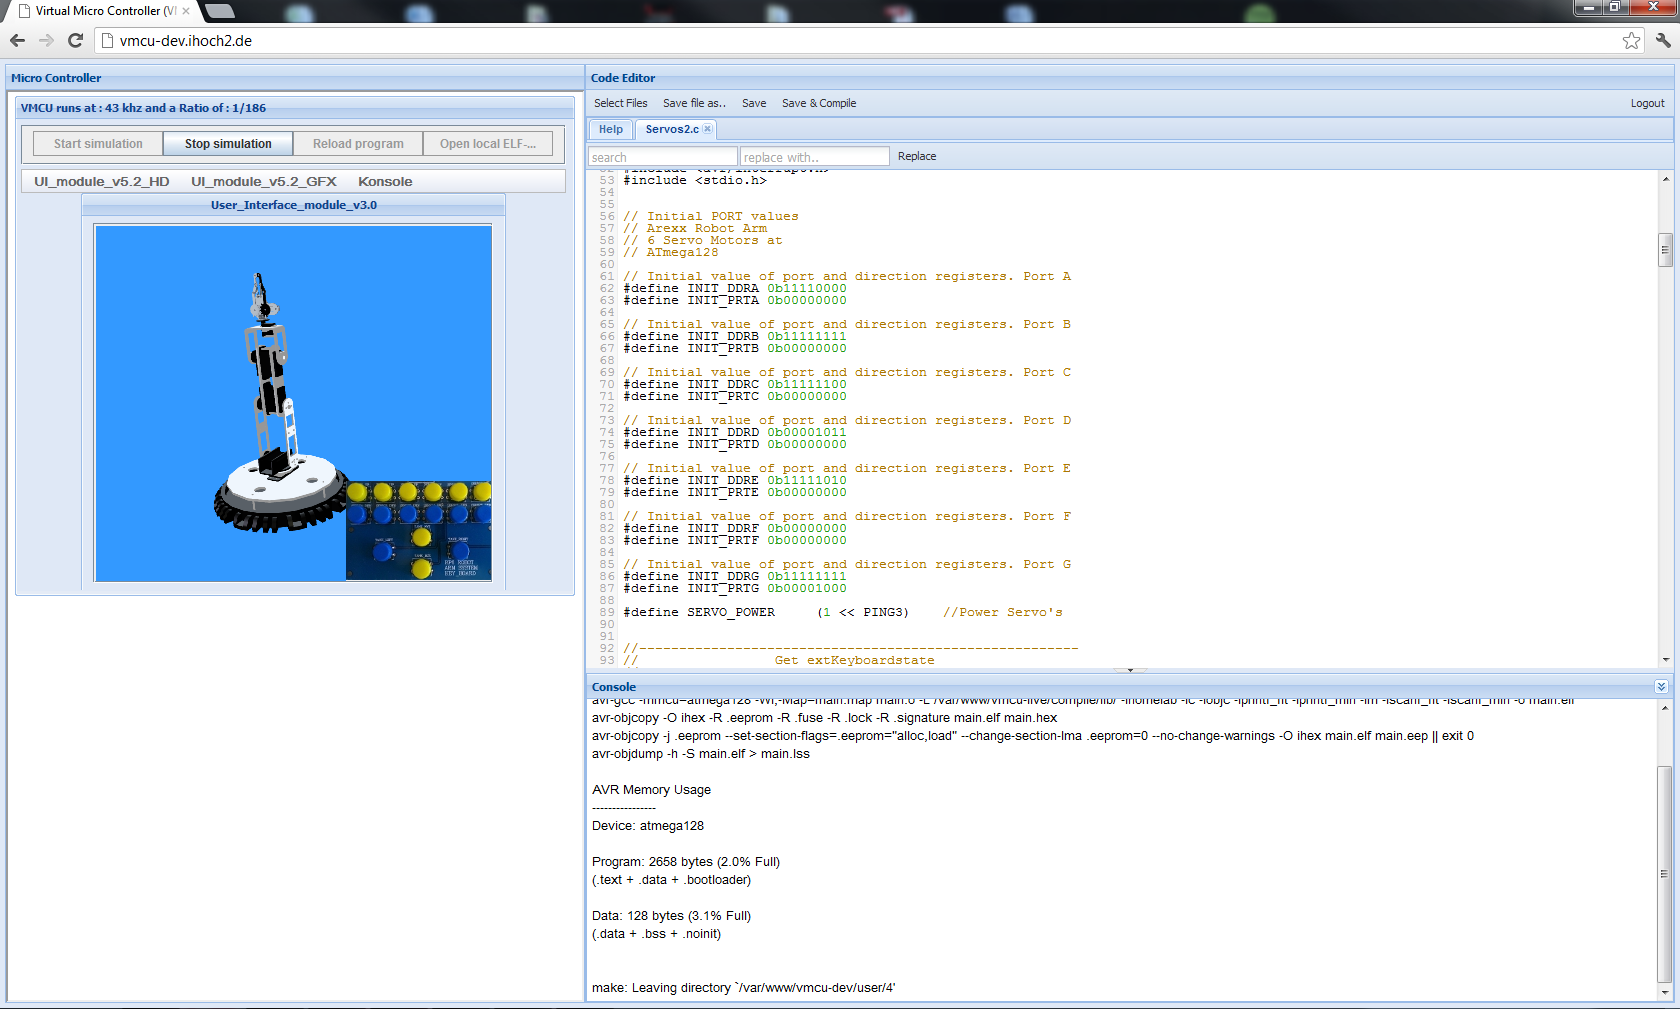
\includegraphics[width=3cm, angle=90]{source/images/vmcu-env}
\caption{3cm breit, 90� gedreht}
\label{fig:dl2:1}
\end{figure}


\begin{figure}[ht]
\begin{minipage}[t]{0.5\textwidth}
\centering
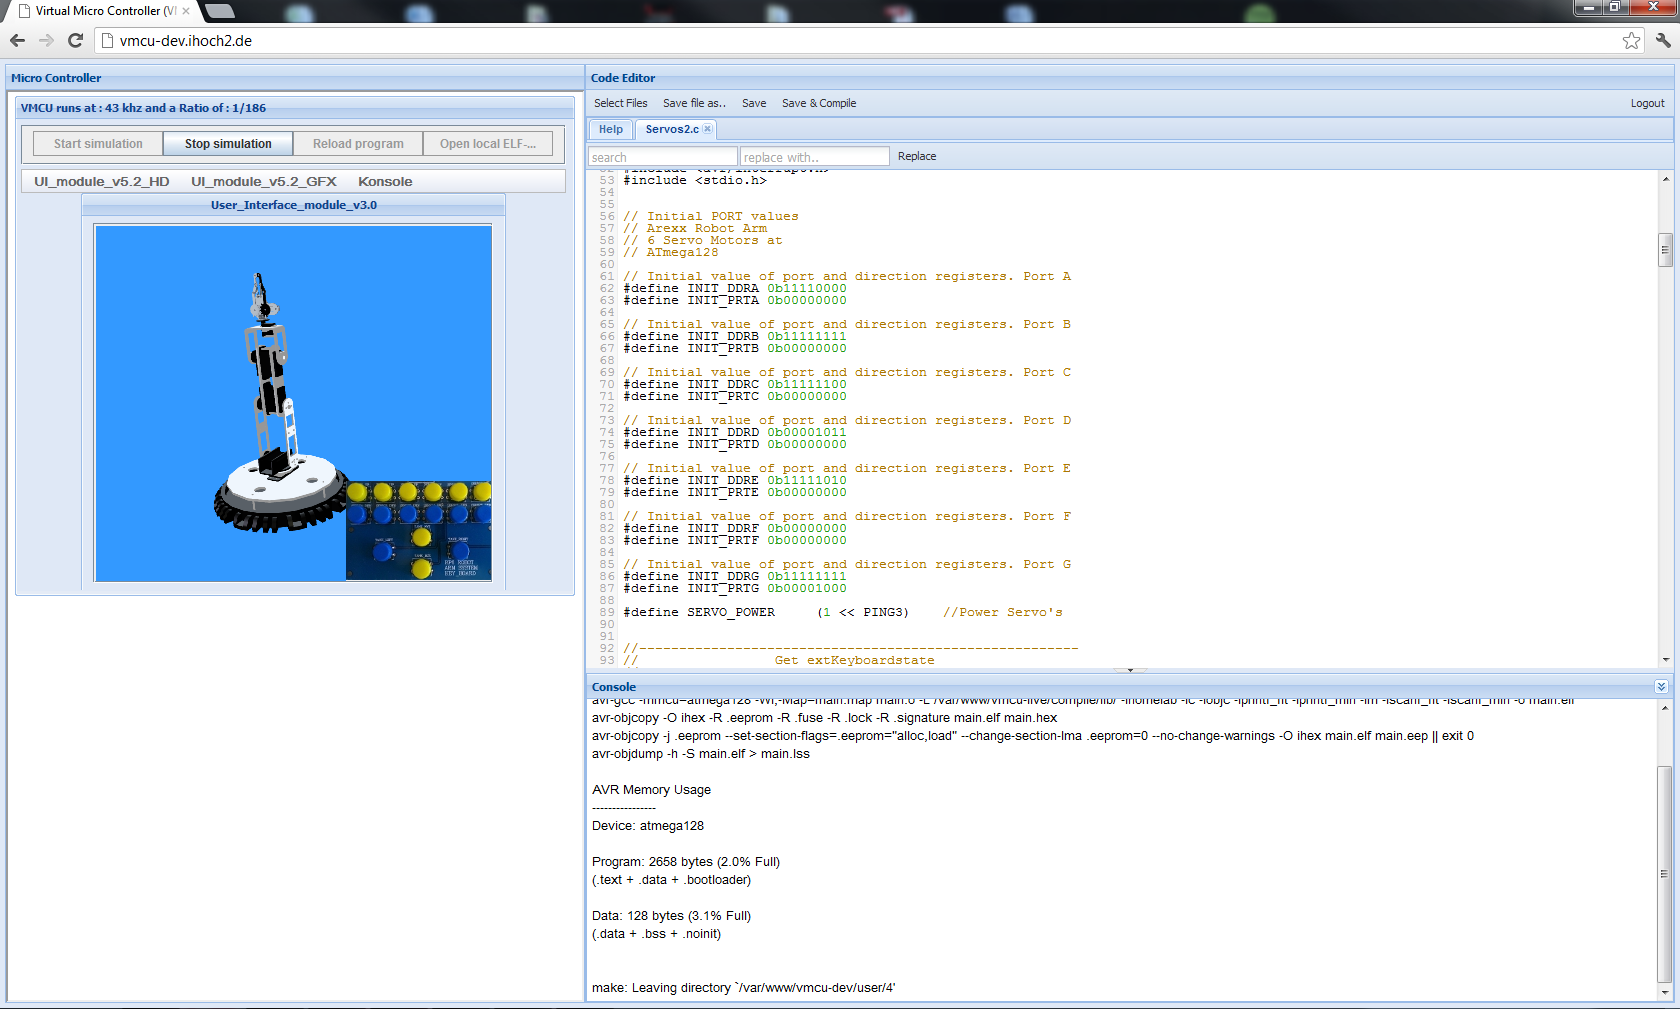
\includegraphics[width=\textwidth]{source/images/vmcu-env}
\caption{links, 40\% d. Textweite}
\label{fig:vmcu:overview3}
\end{minipage}
\hspace{0.5cm}
\begin{minipage}[t]{0.5\textwidth}
\centering
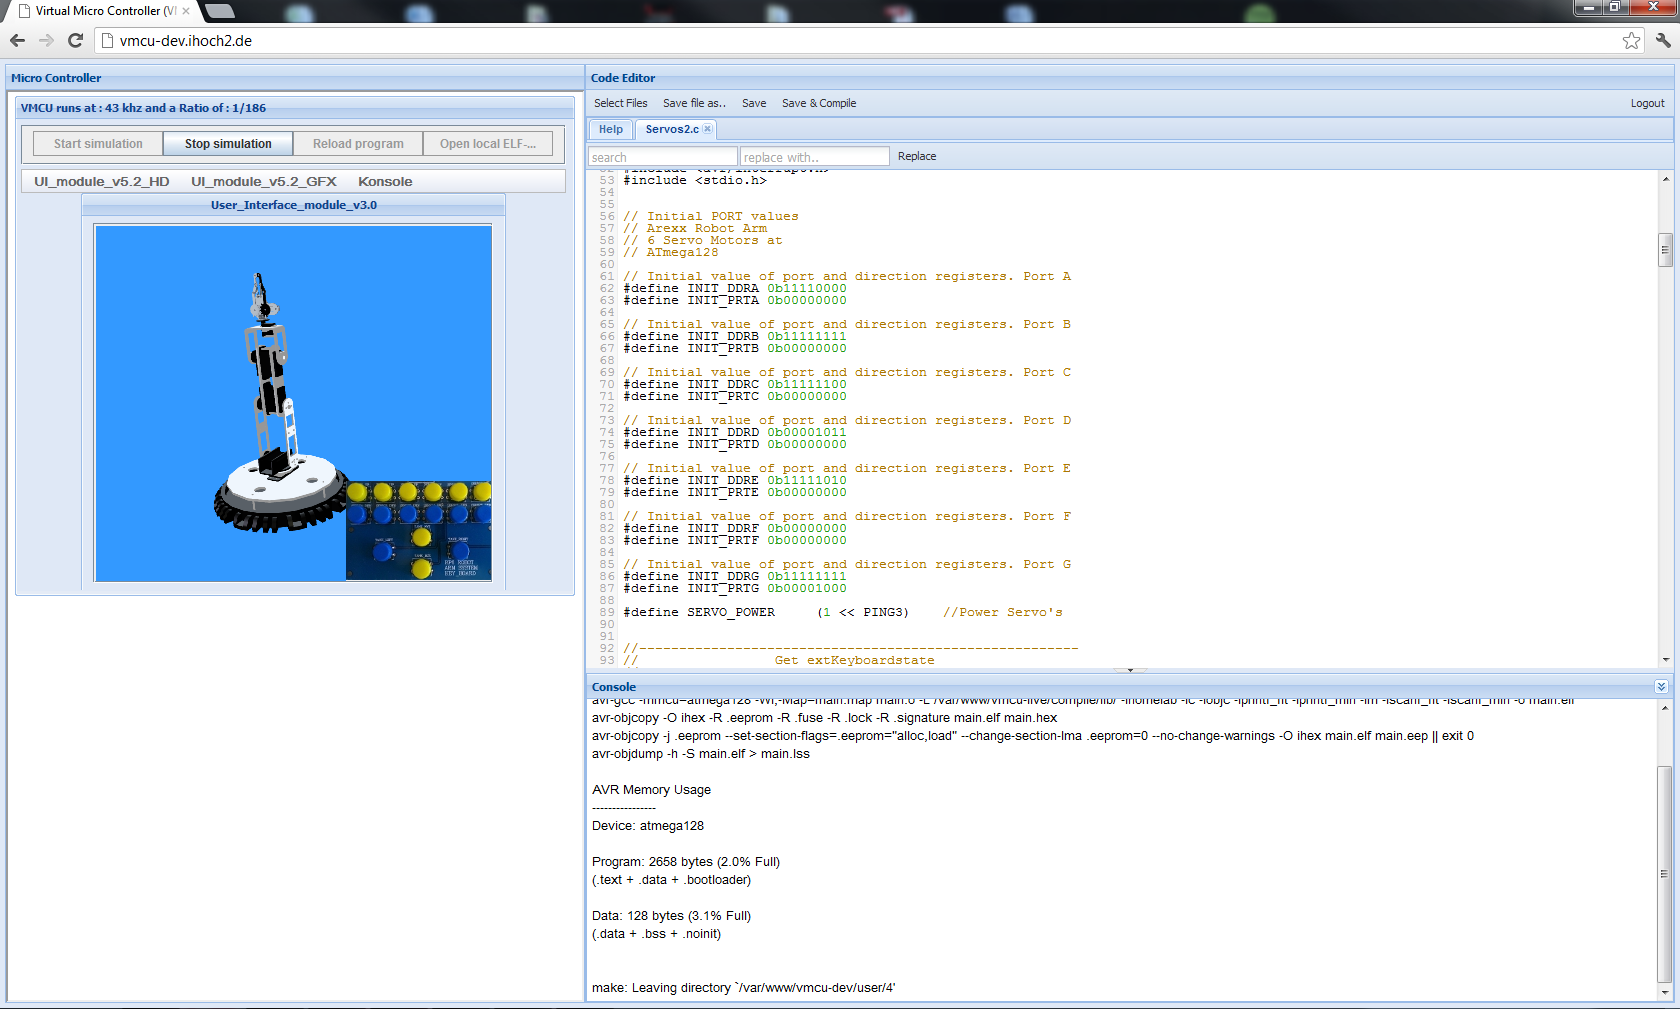
\includegraphics[width=\textwidth]{source/images/vmcu-env}
\caption{rechts, 40\% d. Textweite}
\label{fig:vmcu:overview4}
\end{minipage}
\end{figure}


\section{Tabellen}
Die nachfolgenden beiden Tabellen-Beispiele sind der Internetseite \url{http://en.wikibooks.org/wiki/LaTeX/Tables} entnommen.

Die folgende Tabelle stammt aus \url{http://www.maths.leeds.ac.uk/latex/TableHelp1.pdf}
Sie sehen, dass um das \textit{tabular} ein \textit{table}-Element eingef�gt wurde. Mit diesem k�nnen Sie die Tabelle platzieren und den Umbruch bestimmen. Diese Tabelle taucht auch im Tabellenverzeichnis am Anfang der Arbeit auf! Nutzen Sie daf�r \textit{caption}.

\begin{table}[ht]
\caption{Nonlinear Model Results} % title of Table
\centering % used for centering table
\begin{tabular}{c c c c} % centered columns (4 columns)
\hline\hline %inserts double horizontal lines
Case & Method\#1 & Method\#2 & Method\#3 \\ [0.5ex] % inserts table
%heading
\hline % inserts single horizontal line
1 & 50 & 837 & 970 \\ % inserting body of the table
2 & 47 & 877 & 230 \\
3 & 31 & 25 & 415 \\
4 & 35 & 144 & 2356 \\
5 & 45 & 300 & 556 \\ [1ex] % [1ex] adds vertical space
\hline %inserts single line
\end{tabular}
\label{table:nonlin} % is used to refer this table in the text
\end{table}

Lorem ipsum dolor sit amet, consetetur sadipscing elitr, sed diam nonumy eirmod tempor invidunt ut labore et dolore magna aliquyam erat, sed diam voluptua. At vero eos et accusam et justo duo dolores et ea rebum. Stet clita kasd gubergren, no sea takimata sanctus est Lorem ipsum dolor sit amet. Lorem ipsum dolor sit amet,\\

\begin{tabular}{l*{6}{c}r}
Team              & P & W & D & L & F  & A & Pts \\
\hline
Manchester United & 6 & 4 & 0 & 2 & 10 & 5 & 12  \\
Celtic            & 6 & 3 & 0 & 3 &  8 & 9 &  9  \\
Benfica           & 6 & 2 & 1 & 3 &  7 & 8 &  7  \\
FC Copenhagen     & 6 & 2 & 1 & 2 &  5 & 8 &  7  \\
\end{tabular}\\

Lorem ipsum dolor sit amet, consetetur sadipscing elitr, sed diam nonumy eirmod tempor invidunt ut labore et m ipsum dolor sit amet. Lorem ipsum dolor sit amet, \\

\begin{tabular}{llr}
\hline
\multicolumn{2}{c}{Item} \\
\cline{1-2}
Animal & Description & Price (\$) \\
\hline
Gnat  & per gram & 13.65 \\
      & each     &  0.01 \\
Gnu   & stuffed  & 92.50 \\
Emu   & stuffed  & 33.33 \\
Armadillo & frozen & 8.99 \\
\hline
\end{tabular}





	
\section{Texte}
Das Listing \ref{java1} auf Seite \pageref{java1} zeigt einen Beispielauszug einer \enquote{SQL}-Verbindung aus. Ferner ist in Grafik \ref{fig:vmcu:overview4} der \enquote{Virtual Micro Controller} (VMCU) zu sehen. Aus den beiden Quellen \citep[23]{Sell2009a}, \citep[1]{Seiler20112}, \cite{Sell2011} und \cite{Seiler2011a} geht hervor, dass moderne eLearning-Umgebungen heutzutage aus der Lehre nicht mehr wegzudenken sind. Wie beschrieben, kann gerade im technischen Bereich von internetgest�tzten Plattformen profitiert werden. 

Lorem ipsum dolor sit amet, consetetur sadipscing elitr, sed diam nonumy eirmod tempor invidunt ut labore et dolore magna aliquyam erat, sed diam voluptua. At vero eos et accusam et justo duo dolores et ea rebum. Stet clita kasd gubergren, no sea takimata sanctus est Lorem ipsum dolor sit amet. Lorem ipsum dolor sit amet, consetetur sadipscing elitr, sed diam nonumy eirmod tempor invidunt ut labore et dolore magna aliquyam erat, sed diam voluptua. At vero eos et accusam et justo duo dolores et ea rebum. Stet clita kasd gubergren, no sea takimata sanctus est Lorem ipsum dolor sit amet. Lorem ipsum dolor sit amet, consetetur sadipscing elitr, sed diam nonumy eirmod tempor invidunt ut labore et dolore magna aliquyam erat, sed diam voluptua. At vero eos et accusam et justo duo dolores et ea rebum. Stet clita kasd gubergren, no sea takimata sanctus est Lorem ipsum dolor sit amet. 

Duis autem vel eum iriure dolor in hendrerit in vulputate velit esse molestie consequat, vel illum dolore eu feugiat nulla facilisis at vero eros et accumsan et iusto odio dignissim qui blandit praesent luptatum zzril delenit augue duis dolore te feugait nulla facilisi. Lorem ipsum dolor sit amet, consectetuer adipiscing elit, sed diam nonummy nibh euismod tincidunt ut laoreet dolore magna aliquam erat volutpat. 


\section{To Do Notes}

\tdu{Ein Beispiel-Todo}
\td{und noch ein Todo}
Die Todo Notes lassen sich in der Datei "header.tex" deaktivieren. Dort sind auch die Farben etc. definiert.
\begin{verbatim}
\usepackage[color=red, shadow]{todonotes}
\end{verbatim}

\section{Listings}

\lstinputlisting[language=XML-changed,caption=Beschreibung eines GFX Displays, label=xml1]{source/listings/bsp.xml}
\lstinputlisting[language=Java, firstline=3, lastline=10,caption=Ausschnitte aus dem Java Source Code,label=java2]{source/listings/bsp.java}
\newpage
\lstinputlisting[language=Java,caption=Ein Java Source Code,label=java1]{source/listings/bsp.java}

\section{PDF Dokumente einbinden}
Mit dem Befehl \lstinline[language=Tex]$\includepdf[parameter]{bsp.pdf}$ lassen sich PDF-Dokumente direkt einbinden.
\includepdf[pagecommand={}, pages=-, frame=true, scale=0.68]{source/pdf/bsp.pdf}



%\include{source/content/Test}

%Das Fazit
\chapter{Fazit}
\section{Zusammenfassung}
Was wurde im Rahmen umgesetzt? Anteil der eigenen Entwicklung, Abgrenzung gegen�ber Fremdleistungen

\section{Ausblick}
Wie sieht die Weiterentwicklung aus? Welche M�glichkeiten der Erweiterung / Verbesserung bietet das neue Verfahren / die Software?
%Einbinden des Abbildungsverzeichnisses

\backmatter
%Liste der Tabellen
\listoftables
%Einbinden des Tabellenverzeichnisses
\listoffigures
%Einbinden des Sourcecodeverzeichnisses
\lstlistoflistings

% Quellenverzeichnis
\bibliographystyle{plain}
\bibliography{source/bib/references}

% Anhang
\appendix
\chapter{Danksagung}
Dieser Text bietet sich an f�r eine Danksagung. Bei Bachelorarbeiten ggf. auskommentieren...
\todo[inline]{Danksagung noch erweitern.}
%
% EOF
%

\end{document}



%
% EOF
%